\documentclass[tikz,border=4pt]{standalone}
\usepackage{amsmath,amssymb}
\usetikzlibrary{arrows.meta,decorations.pathmorphing}

\begin{document}
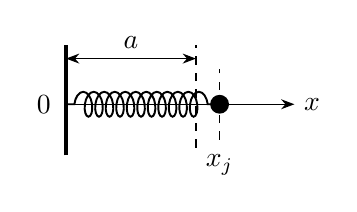
\begin{tikzpicture}[
  >=Stealth,
  font=\normalsize,
  axis/.style={line width=0.4pt},
  curve/.style={line width=0.9pt},
  spring/.style={line width=0.7pt,decorate,decoration={coil,amplitude=4.5pt,segment length=3.8pt,pre length=3pt,post length=3pt}}
]
  % Wall at x = 0
  \draw[line width=1.4pt] (0,-0.65) -- (0,0.75);
  \node[left=2pt] at (0,0) {$0$};

  % Axis
  \draw[axis,->] (0,0) -- (2.9,0) node[right] {$x$};

  % Equilibrium position dashed line at x = 1.65
  \draw[axis,dashed] (1.65,-0.55) -- (1.65,0.75);
  \draw[axis,<->] (0,0.58) -- (1.65,0.58) node[midway,above] {$a$};

  % Spring and mass at x_j = 1.95
  \draw[spring] (0,0) -- (1.95,0);
  \fill (1.95,0) circle (3.4pt);
  \draw[axis,dashed] (1.95,-0.45) -- (1.95,0.45);
  \node[below=2pt] at (1.95,-0.45) {$x_j$};
\end{tikzpicture}
\end{document}
